\begin{figure*}[t!]
    \centering
        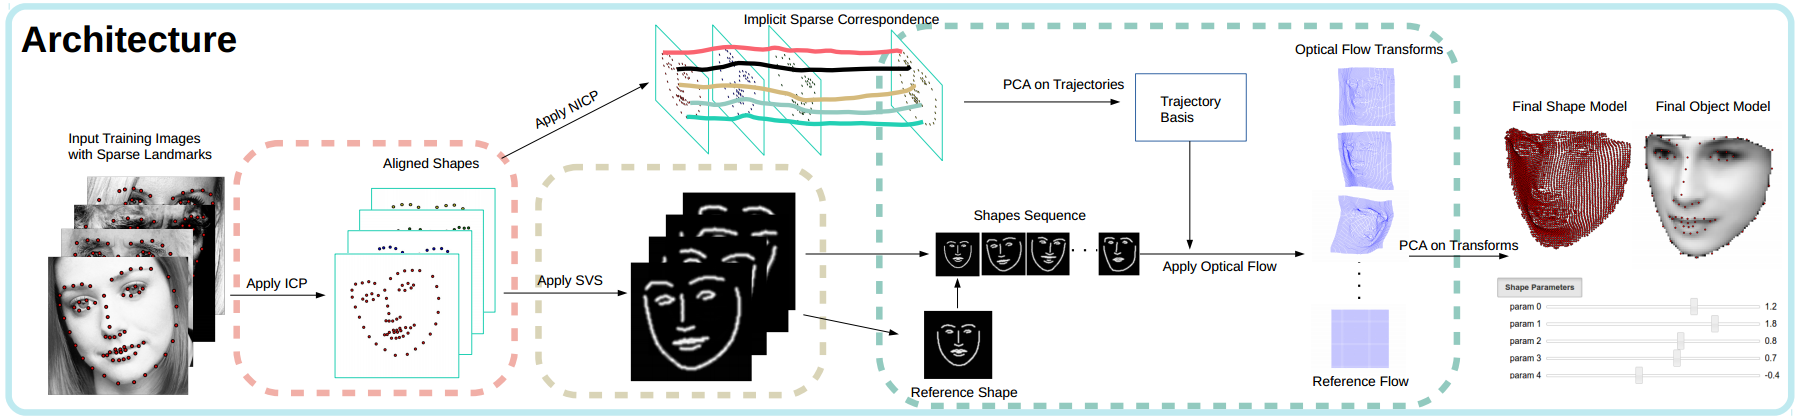
\includegraphics[width=\textwidth]{resources/architecture}
    \caption{Proposed pipeline.}
    \label{fig:archi}
\end{figure*}

\section{Deformable Models without Landmarks}

% Deformable models are widely used for object detection, localization, recognition and tracking while training a deformable model with good generalisation requires tremendous amount of carefully annotated data, which is extremely time consuming. Even more, annotated data of a specific object category typically requires same numbers of landmarks for every training sample, making the annotation procedure significantly complex where corrext menual annotation of landmarks is impossible in various object classes e.g. ears.

% Despite the fact that that vast majority of existing methods are based on a sparse shape representation, dense shape representation reveals more nuanced structure in terms of [todo: explain].

We propose a novel framework for building deformable models that does not require any consistent set of annotated landmarks and is based on a dense shape representation. Our method only requires a set of point or curve line annotations that does not need to be consistent over different training samples. It combines the techniques of Non-rigid Iterative Closest Point (NICP) \cite{Amber2007}, multi-channel Support Vector Shape (SVS) \cite{Nguyen2013} representation and multi-image subspace flow \cite{Garg:2013hu} in an effective framework that has significant descriptive power.

The proposed pipeline is depicted in Figure~\ref{fig:archi}. It takes as input a set of training images of a particular object class, along with (possibly inconsistent) point and/or curve line annotations. 
As a first step, the shapes that correspond to the training data are consistently represented using multichannel SVS. 
The next step is the application of ICP to achieve an initial simple alignment of the SVS images. 
The similarity-aligned SVS images are then fed into a multi-image subspace flow estimation that establishes dense correspondences between all shapes of the training set. In order for the flow estimation to be accurate and exploit the correlation across the different training shapes, it utilises a correspondence basis that is built on sparse correspondences given by Nonrigid ICP alignment of the annotated data. Finally, the dense correspondences that are yielded by the optical flow serve as automatic dense landmarks and are used to define a novel dense version of Active Appearance Models. The following sections discuss the different stages of the proposed pipeline in further detail.

%two major modules. The first module handles inconsistent annotation set by converting to landmark independent shape discriminator. While the other module produces shape flow on object discriminators to generate dense flow transformations in shape space following by robust PCA\cite{?} to generate deformable model. In this section, we present the entire architectures, design decision and algorithms.
\subsection{Shape Representation Without Consistent Annotations}
\label{sec:svs}
%Ordinarily, construction of deformable model requires training data set having consistent number of landmarks. But unavoidable changes has to be made before applying same algorithm on diverse annotated data set.

In order to fully capture the variability among most deformable object shapes annotations, we use a representation based on Support Vector Shapes (SVS) \cite{Nguyen2013}. An SVS is a decision function trained on shapes using Support Vector Machines (SVMs) with  Radial Basis Function (RBF) kernels. In this way, a shape is represented as a classifier function, which has several advantages: (a) The representation is completely general, \eg it can be applied to sparse landmark points, curves lines or a combination of the two and (b) It fuses inconsistent landmarks into consistent and directly comparable decision functions. Furthermore, this representations is also robust against noise, missing data and outliers.

In practice, we assume that all the training images correspond to the same object category and contain a set of inconsistent points and curve line annotations. All annotations are densely sampled to yield a set of annotated landmarks per image, with this set being different for every training image. Initially, negative points get randomly sampled around sparse landmarks while annotated landmarks are positive points. Since the number of positive points is far smaller that the number of negative ones, landmarks are assigned considerably larger weights so that $N_p \times W_p=N_n \times W_n$ where $N_p, N_n$ are number of positive/negative samples and $W_p, W_n$ are their corresponding weights.

SVMs with RBF kernel function map any numbers of data points onto an infinite-dimensional space where positive and negative points are linearly separable, hence the classification boundary on 2D space represents the actual shape of the object. Note that the decision function for SVMs can be mathematically expressed as:
\begin{equation} \label{eq:decisionfunc}
    d(\mathbf{x})=\sum_i\alpha_i \, k(\mathbf{x}_i^*,\mathbf{x})
\end{equation}
where $\mathbf{x}_i^*$ are support vectors and \mbox{$k(\mathbf{x}_i^*, \mathbf{x}) = exp(-\lambda \|\mathbf{x}_i^* -\mathbf{x}\|^2)$} is the RBF kernel .

Figure \ref{fig:build_svs} shows an exemplar shape representation using SVS. As it can be observed, the final result does not drastically depend on the original number of annotated landmarks.


\begin{figure}[b!]
    \centering
    \begin{subfigure}[b]{0.2\textwidth}
            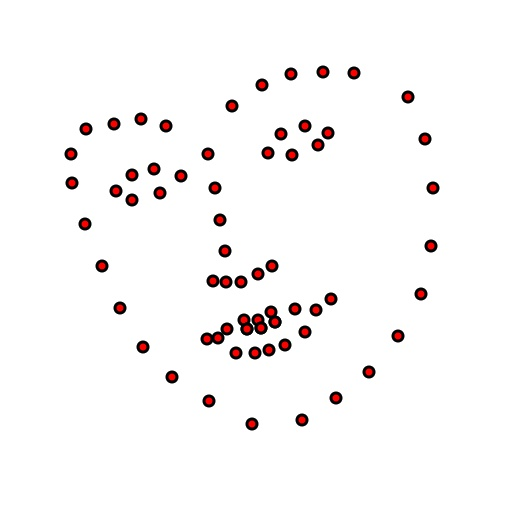
\includegraphics[width=\textwidth]{resources/landmark}
        \caption{Spare landmarks}
    \end{subfigure}
    \qquad
    \begin{subfigure}[b]{0.2\textwidth}
            
\includegraphics[width=\textwidth]{resources/svs}
        \caption{Decision function}
        \label{fig:svs}
    \end{subfigure}
    \caption{Exemplar SVS shape representation. The decision function is trained on the set of sparse landmarks. In (b), brighter colour represents higher probability of a pixels belonging to the original shape.}
    \label{fig:build_svs}
\end{figure}


After constructing the SVS representation for all images, the next step is to apply a simple similarity alignment over them. This is done because the goal here is to build a model capable of effectively representing non-rigid local shape deformations rather than global rotation, translation and scaling. The alignment is performed by using the Iterative Closest Point (ICP) algorithm \cite{Besl1992} on the annotated landmarks point cloud of the training images.


\subsection{Shape Correspondence Basis}

In order to robustly establish dense correspondences across all SVS images using optical flow, it is important to constrain how pixels are allowed to move from one SVS image to another. In this work, we constrained the range of allowed pixels movements by learning a correspondence subspace. 

In order to learn such a subspace, we first transform the original annotation to point clouds. Then, we use NICP to align the previous point clouds with respect to a reference point cloud template. NICP iteratively deforms each point cloud until its points match the ones on the shape template and correspondences are established. However, because optical flow is a pixel-wise frame registration technique, we need to establish correspondences for all pixels on the reference frame rather than for sparse point clouds. To achieve this, we apply Thin Plate Spline (TPS) \cite{Bookstein1989} to find correspondences for all pixels in the reference frame given the point cloud correspondences provided by the previous NICP stage. Once dense correspondences have been established among all pixels, the so-called correspondence subspace is obtained by performing PCA the trajectory of all pixels. Note that incorporating the previous subspace as a low rank constrained in optical flow is consistent with its assumption of smooth motion.

% For all dense transformations $\bm{u_n}(\bm{x}), n \in \{1,...,F\}$, where $F$ is number of data and $\bm{x}$ is vector of pixels, Principle Component Analysis (PCA) is performed on trajectory to obtain low rank trajectory basis:
% \begin{equation}
%     \begin{bmatrix}
%         \bm{u_1}(\bm{x}) \\
%         \vdots \\
%         \bm{u_F}(\bm{x})
%     \end{bmatrix}
%     =
%     \begin{bmatrix}
%         \bm{q_1}(1) & \cdots & \bm{q_R}(1) \\
%         \vdots      & \ddots & \vdots  \\
%         \bm{q_1}(F) & \cdots & \bm{q_R}(F)
%     \end{bmatrix}
%     \times
%     \begin{bmatrix}
%         \bm{v_1}(x) \\
%         \vdots \\
%         \bm{v_R}(x)
%     \end{bmatrix}
% \end{equation}
% where $\bm{q_i}(n)$ are low rank components with $R \ll 2F$ and $\bm{v_i}(x)$ weighted each component with dependencies on $x$. Simpler expression shown below:
% \begin{equation}
%     \bm{u_n}(\bm{x})=\sum_{i=1}^R\bm{q_i}(n)\bm{v_i}(x)+\bm{\varepsilon_n}(\bm{x})
% \end{equation}


\begin{figure}[t!]
    \centering
    \begin{subfigure}[b]{0.15\textwidth}
            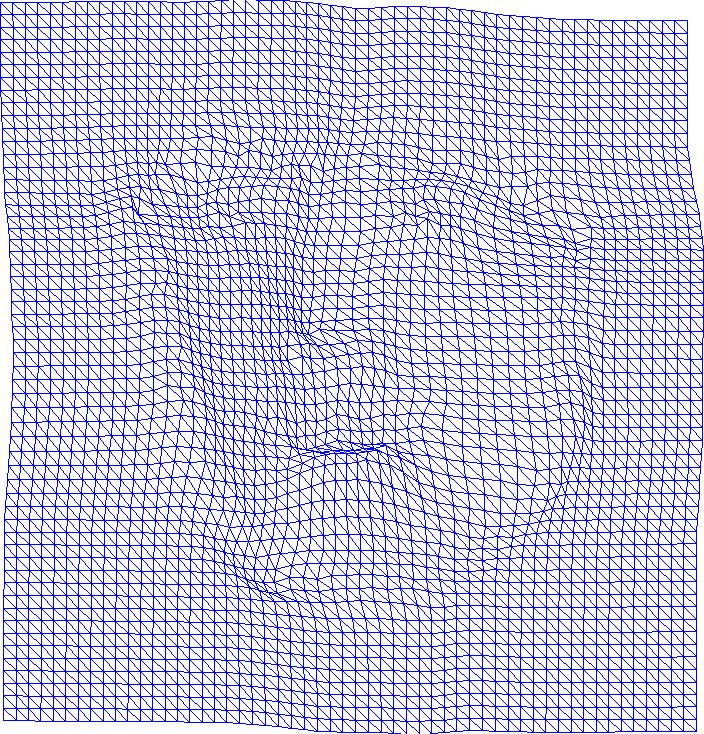
\includegraphics[width=\textwidth]{resources/Fig_Flows/0}
    \end{subfigure}
    \hfill
    \begin{subfigure}[b]{0.15\textwidth}
            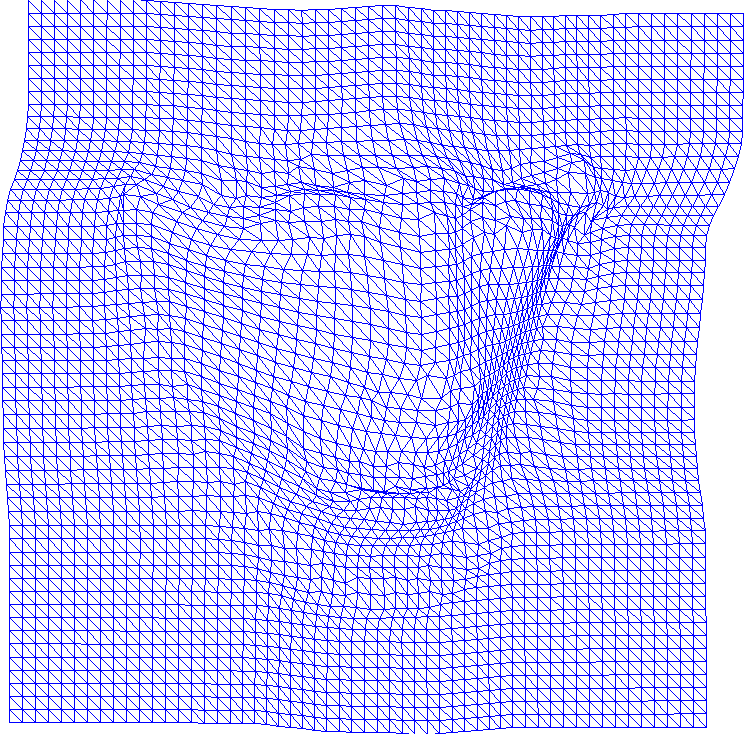
\includegraphics[width=\textwidth]{resources/Fig_Flows/1}
    \end{subfigure}
   	\hfill
    \begin{subfigure}[b]{0.15\textwidth}
            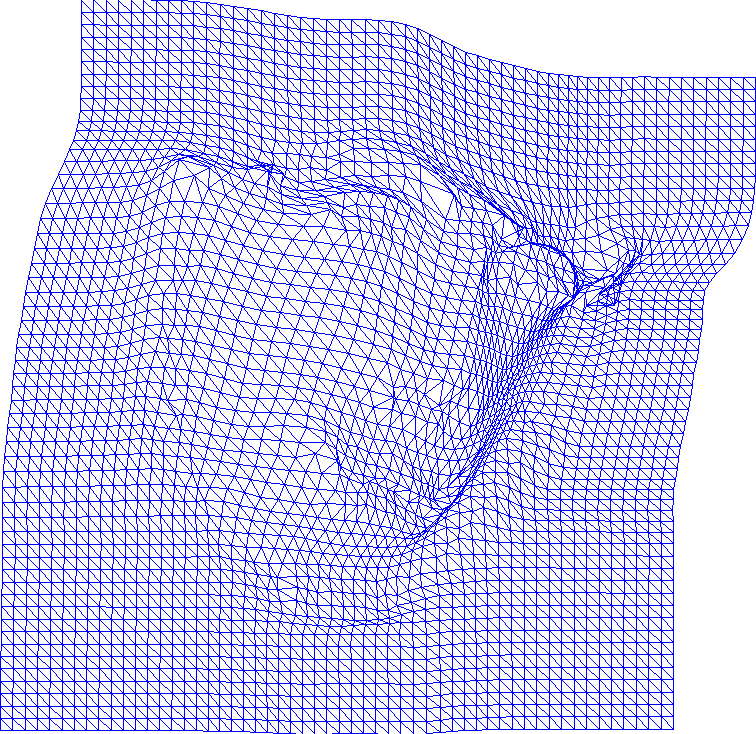
\includegraphics[width=\textwidth]{resources/Fig_Flows/2}
    \end{subfigure}
    \\
    \begin{subfigure}[b]{0.15\textwidth}
            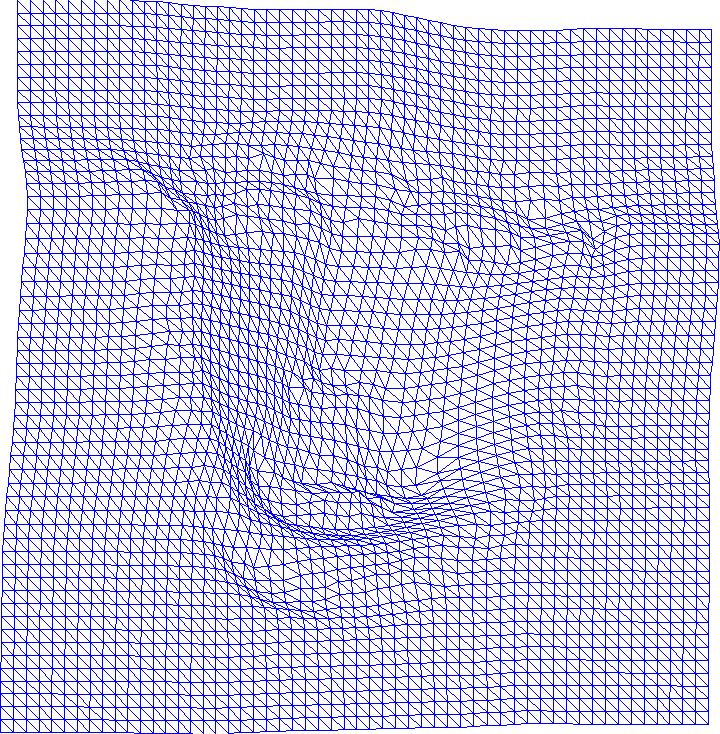
\includegraphics[width=\textwidth]{resources/Fig_Flows/3}
    \end{subfigure}
    \hfill
    \begin{subfigure}[b]{0.15\textwidth}
            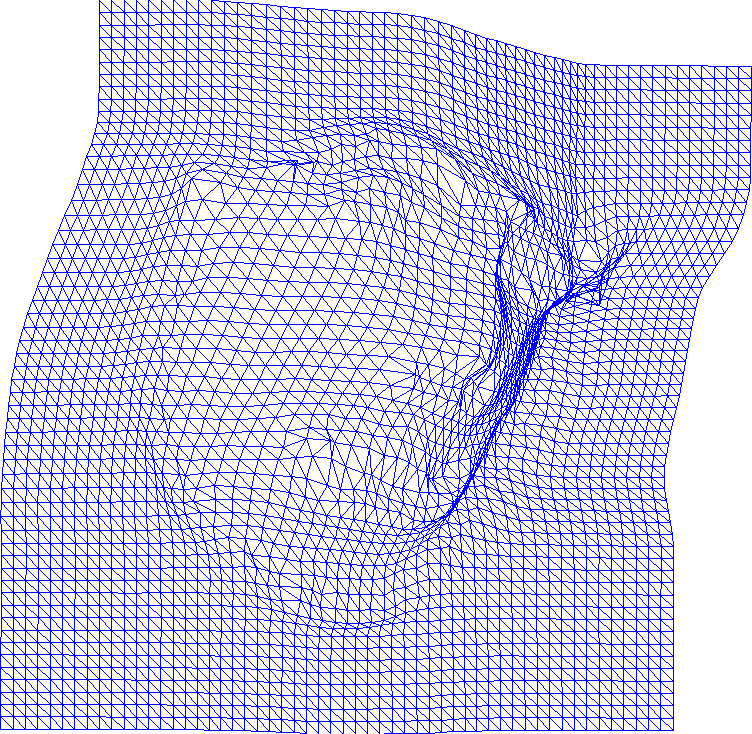
\includegraphics[width=\textwidth]{resources/Fig_Flows/4}
    \end{subfigure}
   	\hfill
    \begin{subfigure}[b]{0.15\textwidth}
            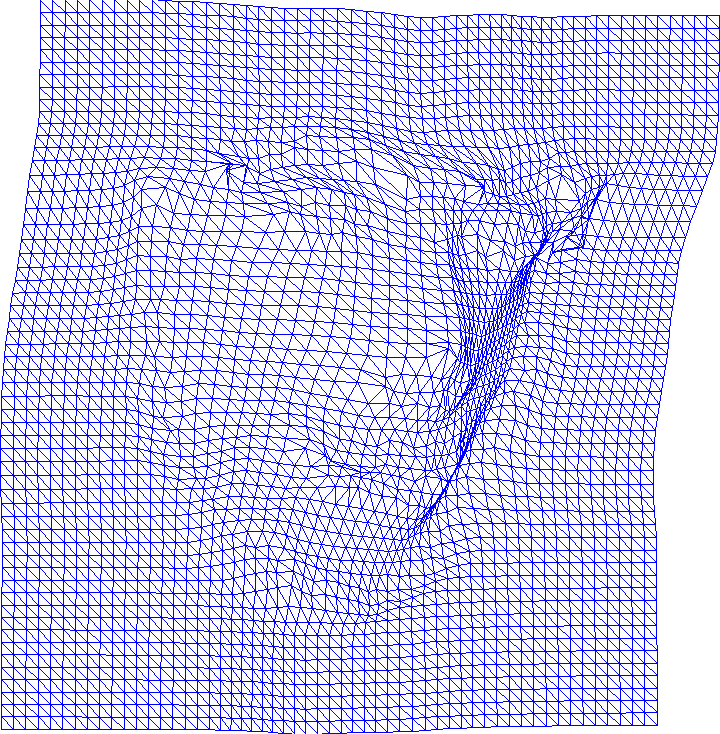
\includegraphics[width=\textwidth]{resources/Fig_Flows/5}
    \end{subfigure}
    \\
    \begin{subfigure}[b]{0.15\textwidth}
            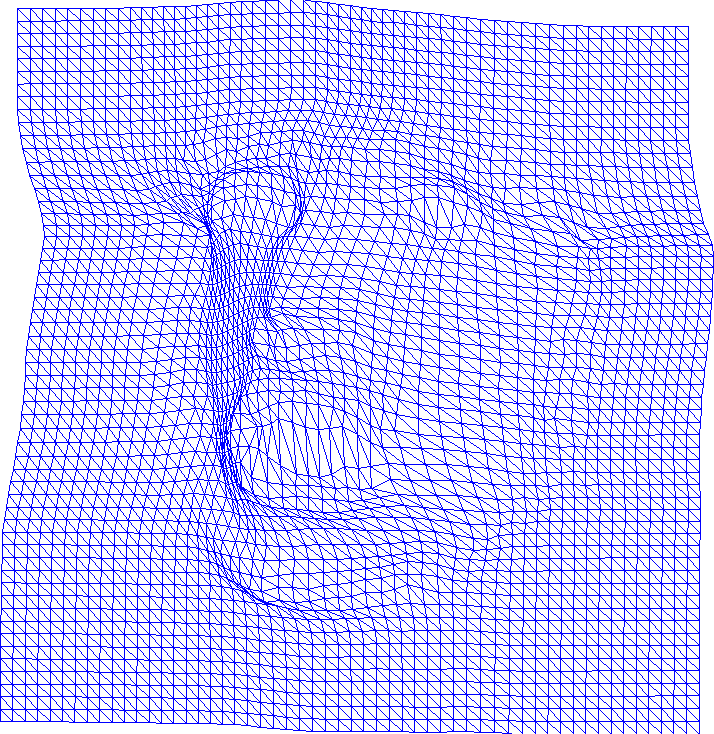
\includegraphics[width=\textwidth]{resources/Fig_Flows/6}
    \end{subfigure}
    \hfill
    \begin{subfigure}[b]{0.15\textwidth}
            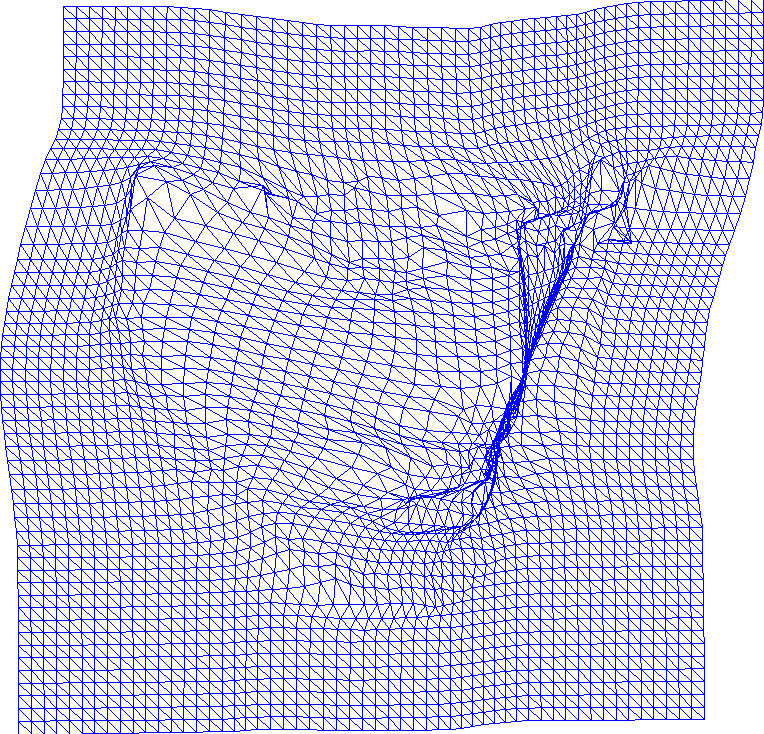
\includegraphics[width=\textwidth]{resources/Fig_Flows/7}
    \end{subfigure}
   	\hfill
    \begin{subfigure}[b]{0.15\textwidth}
            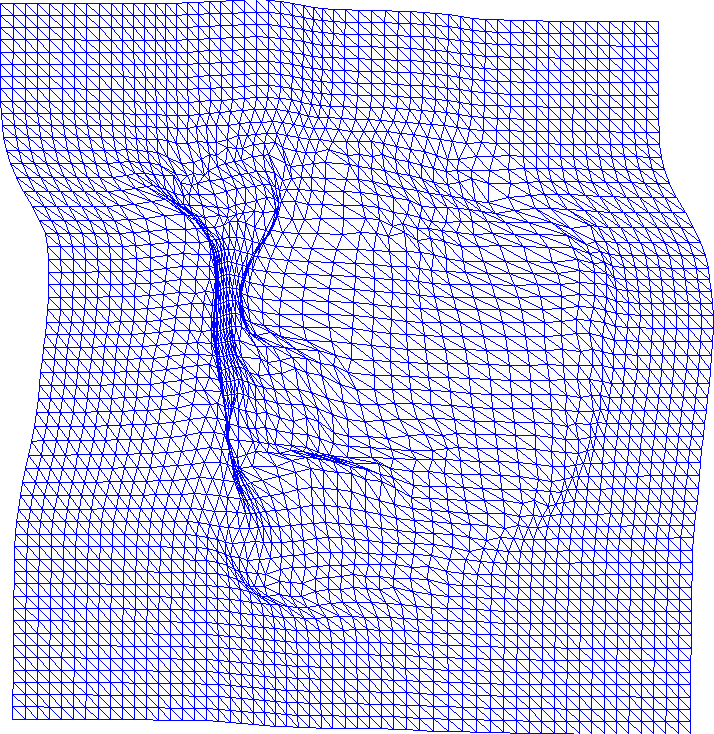
\includegraphics[width=\textwidth]{resources/Fig_Flows/8}
    \end{subfigure}
    \caption{Deformation field built}
    \label{fig:deformationfield}
\end{figure}




% ---------------------------------------------------------------------------------------------------------------------------------------------------


\subsection{Shape Flow}
\label{sec:shapeflow}

Using the SVS functions built from training data, the next step of our pipeline is to establish dense correspondences between all these functions. We propose to do this procedure jointly, by using the correspondence basis. This procedure shares similarities with multiframe optical flow and we call it Shape flow. We build upon robust methods for  optical flow estimation. Optical flow estimation typically works based on the assumptions of brightness or colour constancy and motion smoothness. However, in terms of shapes, neither constant illumination nor continuous motion exists in sequence of shapes as all training data are independent. 
For this reason, we propose to modify the formulation of multiframe optical flow by using the correspondence basis that we introduced in conjunction with the SVS functions, rather than actual images.

\subsubsection{Non-rigid ICP and Correspondence Basis Creation} \label{sec:trabasis}
Since shapes from training data set having completely no motion smoothness, it is of importance to contain constraints in optimization on how pixels moves from one shape frame to another. We constrain the optimization on correspondence subspace.
We supervise trajectories from sparse landmarks. To begin with, Non-rigid Iterative Closest Point (NICP)\cite{Amber2007} applied on sparse annotated points. NICP deforms target points to fit the template iteratively until all points on target deformed to match points on template. Performs the algorithm for all training data will get an implicit point correlation between sparse shapes.

Since optical flow pixel-wise frame registration, the trajectory basis build should also match the dimension, which is dense on shapes with trajectory length depends on number of training data. With correspondences produced after applying NICP, Thin-Plate Spline (TPS)\cite{Bookstein1989} transformations are utilized to warp every shape planes to template plane thereby generates an implicit dense shape registering. For all dense transformations $\bm{u_n}(\bm{x}), n \in \{1,...,F\}$, where $F$ is number of data and $\bm{x}$ is vector of pixels, Principle Component Analysis (PCA) is performed on trajectory to obtain low rank trajectory basis:
\begin{equation}
    \begin{bmatrix}
        \bm{u_1}(\bm{x}) \\
        \vdots \\
        \bm{u_F}(\bm{x})
    \end{bmatrix}
    =
    \begin{bmatrix}
        \bm{q_1}(1) & \cdots & \bm{q_R}(1) \\
        \vdots      & \ddots & \vdots  \\
        \bm{q_1}(F) & \cdots & \bm{q_R}(F)
    \end{bmatrix}
    \times
    \begin{bmatrix}
        \bm{v_1}(x) \\
        \vdots \\
        \bm{v_R}(x)
    \end{bmatrix}
\end{equation}
where $\bm{q_i}(n)$ are low rank components with $R \ll 2F$ and $\bm{v_i}(x)$ weighted each component with dependencies on $x$. Simpler expression shown below:
\begin{equation}
    \bm{u_n}(\bm{x})=\sum_{i=1}^R\bm{q_i}(n)\bm{v_i}(x)+\bm{\varepsilon_n}(\bm{x})
\end{equation}
Although optical flow on shapes made under the assumption that objects motion are smooth, the low rank constrain on trajectory basis recovered the hypothesis.

\subsubsection{Multi-image Subspace Flow}
To register all decision functions to template shape, decision function $d_i(\bm{x}), i \in {1,...,F}$ are grouped into one sequence before applying flow algorithm. The objective cost function we would like to minimise is:
\begin{align}
    \operatorname*{arg\,min}_{\bm{u_n}(\bm{x}), \bm{v}}&=\alpha \int_{\Omega}\sum_{n=1}^F|\bm{d_n}(x+\bm{u_n}(x))-\bm{d_0}(x)\| dx  \label{eq:costfunc}\\
    &+ \beta \int_{\Omega}\sum_{n=1}^F\|\bm{u_n}(x)-\sum_{i=1}^R\bm{q_i}(n)\bm{v_i}(x)\|^2 dx \label{eq:lowrank}\\
    &+ \sum[\bm{TV}(Qv)] + v^T.L.V
\end{align}
where $d_n(x)$ is the decision function from~\eqref{eq:decisionfunc}, which returns possibilities of given coordinate classified as shape component where coordinates are from set $\Omega \in \Re^2$. $TV(Qv)$ is total variation as regularization on low rank subspace, $Q$ is trajectory basis and $v^T.L.v$ is low rank spacial constraints.

Term~\eqref{eq:costfunc} state the shape constancy where points having similar classification probability are from same object.
Part~\eqref{eq:lowrank} applies constrain on low rank trajectory basis states in section~\ref{sec:trabasis}.
The objective cost function has two free parameters $u$ and $v$, so we perform alternating minimisation. The equation can be solved using a thresholding scheme after linearisation of image functions. The minimisation can be speed up by paralleling the minimisation for every spatial-temporal point $(x;n), x \in \Omega, n \in \{1,...F\}$ independently.

After solving the equation, $\bm{u_n}(\bm{x}), x \in \Omega$ gives a group of deformation fields that registering every decision functions in the shape sequence to reference frame e.g. $\bm{u_1}(\bm{x})$ registers decision function $\bm{d_1}(\bm{x})$ to the reference frame. Figure~\ref{fig:deformationfield} demonstrates deformation fields that warps from reference frame where there is no deformation.

% \begin{figure}[h!]
%     \centering
%         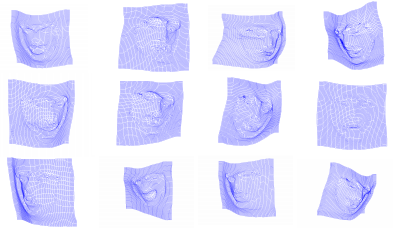
\includegraphics[width=0.5\textwidth]{resources/df}
%     \caption{Deformation field built}
%     \label{fig:deformationfield}
% \end{figure}



Applying PCA on deformations trains dense deformable shape model:
\begin{equation*}
    \bm{s_p}=\bm{\bar{s}} + \bm{U}_s\bm{p}
\end{equation*}
where $\bm{s_p}$ is deformed shape instance. $\bm{\bar{s}}$ is mean shape and $\bm{U}_s\bm{p}$ are eigenvectors with corresponding parameters $p$. Figure~\ref{fig:models} shows an instance of deformed shape and appearance model.
\begin{figure}[h!]
    \centering
    \begin{subfigure}[b]{0.22\textwidth}
            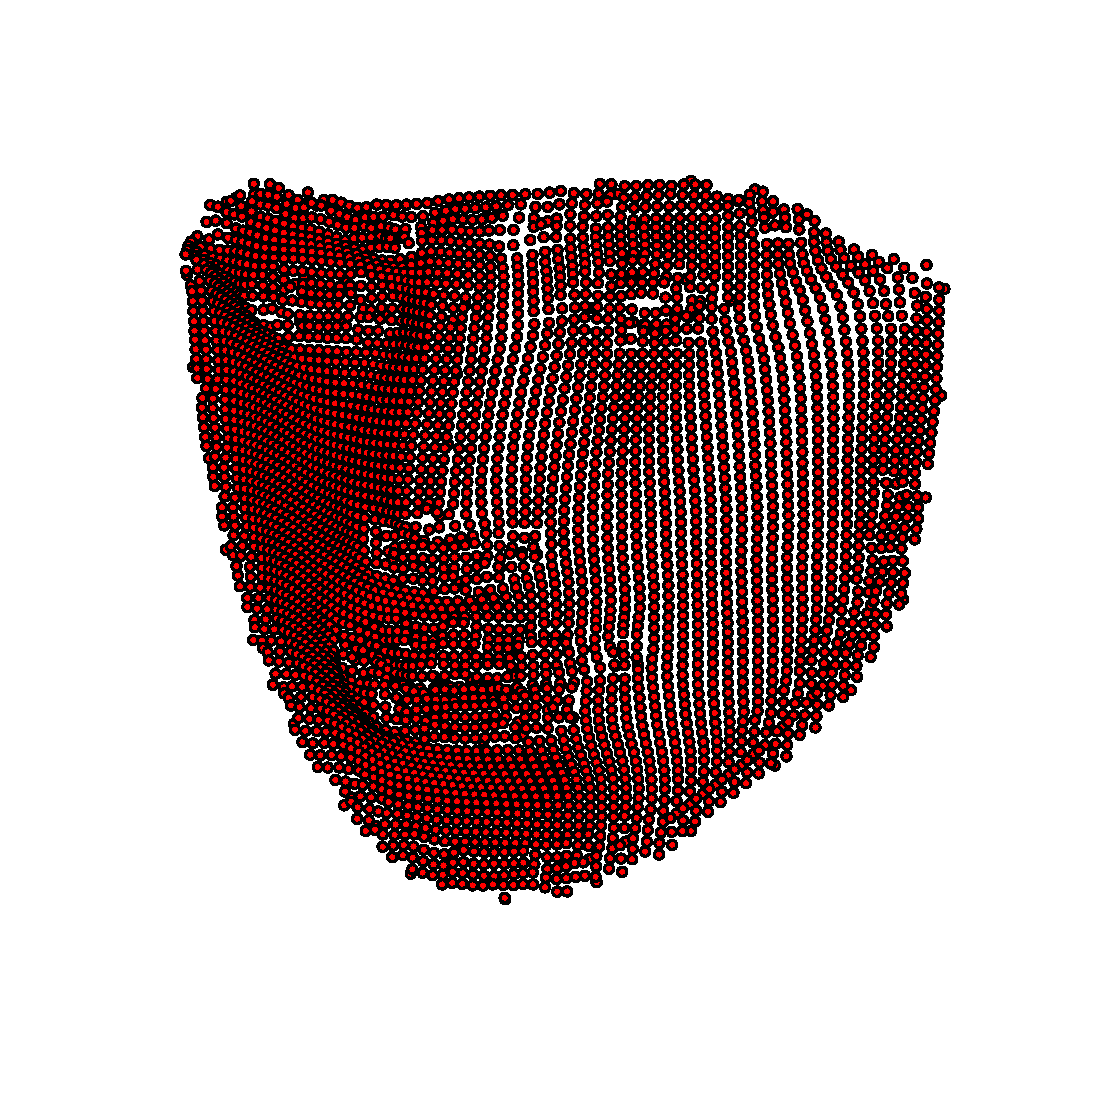
\includegraphics[width=\textwidth]{resources/Fig_dAAM/of_shape}
    \end{subfigure}
  	\hfill
    \begin{subfigure}[b]{0.22\textwidth}
            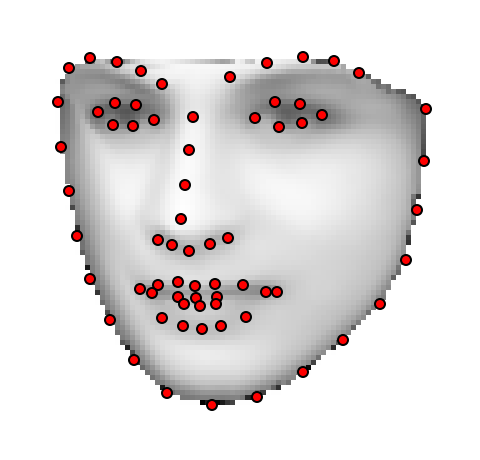
\includegraphics[width=\textwidth]{resources/Fig_dAAM/of_app}
    \end{subfigure}
    \caption{Dense Deformable Model}
    \label{fig:models}
\end{figure}

% \begin{figure}[h!]
%     \centering
%     \begin{subfigure}[b]{0.22\textwidth}
%             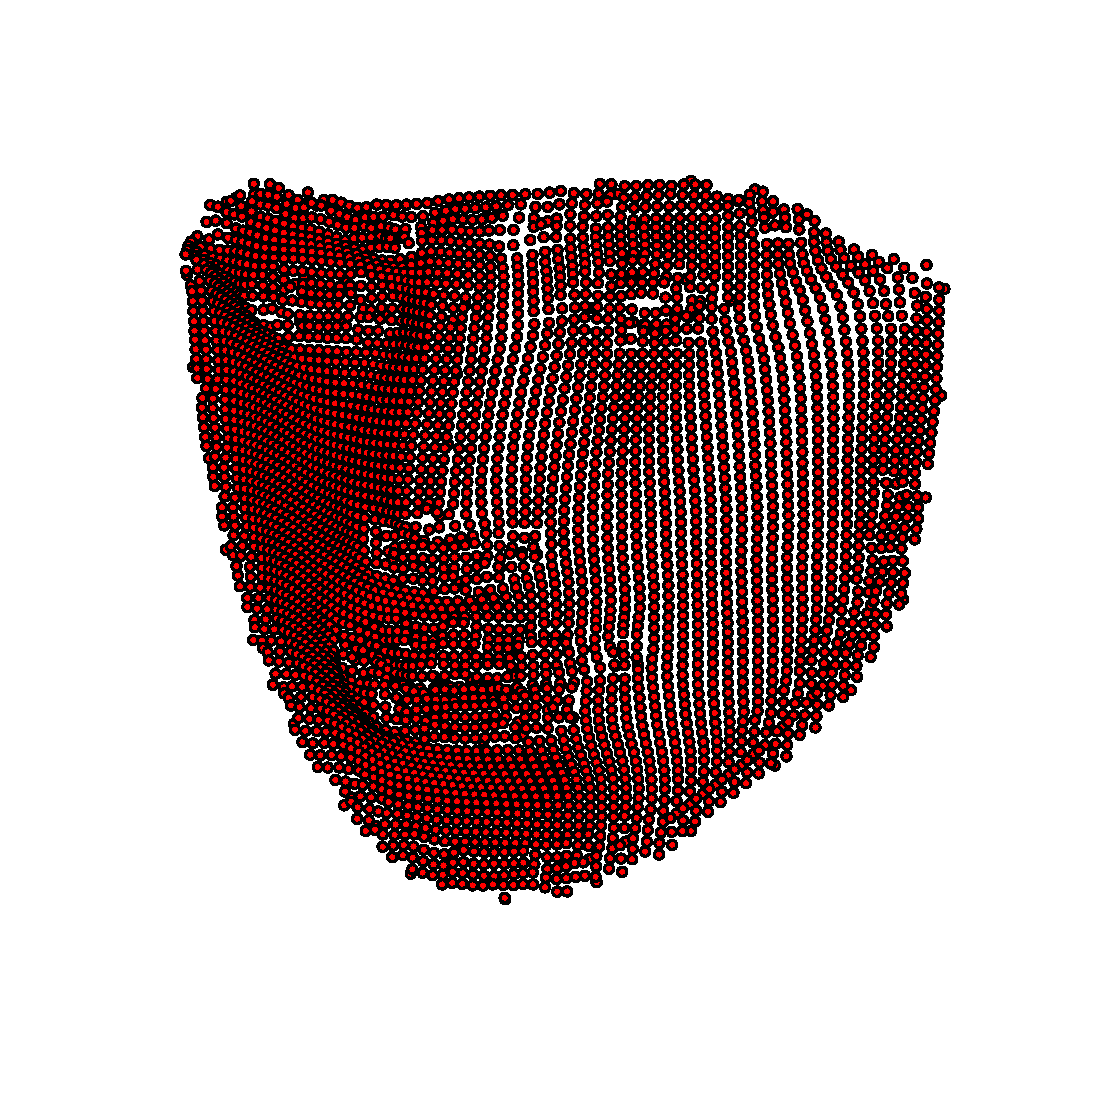
\includegraphics[width=\textwidth]{resources/Fig_dAAM/of_shape}
%     \end{subfigure}
%   	\hfill
%     \begin{subfigure}[b]{0.22\textwidth}
%             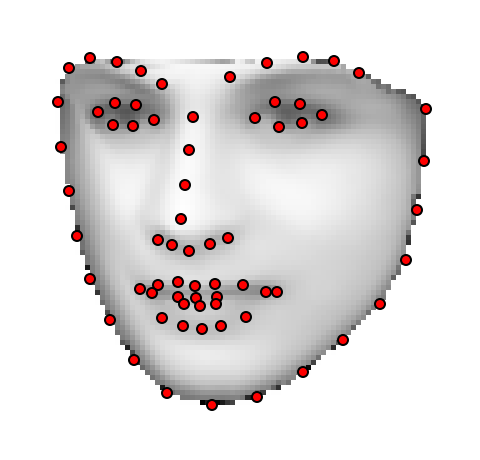
\includegraphics[width=\textwidth]{resources/Fig_dAAM/of_app}
%     \end{subfigure}
%     \caption{Dense Deformable Model}
%     \label{fig:models}
% \end{figure}

\subsection{Dense Active Appearance Models}

The deformation fields obtained in section \ref{sec:shapeflow} can be effectively used to learn a naturally dense version of Active Appearance Models \cite{Cootes2001, Matthews2004}. Because all deformation fields contain the same number of pixels (the same as on the reference frame) the spatial positions $\mathbf{x}_i=(x_i, y_i)$ of these pixels can be treated as point landmarks and the deformation field themselves as dense annotations of the object's shape. Consequently, building a dense shape model reduces to normalizing these dense annotations with respect to a global similarity transform (typically using Procrustes Analysis) and applying Principal Component Analysis (PCA). The resulting shape model can be mathematically expressed as:
\begin{equation}
    \begin{aligned}
        \mathbf{s} & = \mathbf{\bar{s}} + \mathbf{S} \mathbf{p}
    \end{aligned}
    \label{eq:shape_model}
\end{equation}
where $\mathbf{\bar{s}}$ is mean shape and $\mathbf{S}$ and $\mathbf{p}$ are the shape bases and parameters respectively.

On the other hand, the texture model associated to the previous set of densified shapes can be easily obtained by warping all image onto the reference frame, making explicit use of the one-to-one correspondence between pixels on the reference frame and on the deformation fields. Once the images have been warped, the texture model is obtained by applying PCA on the warped images. The texture model is mathematically defined by the following expression:
\begin{equation}
    \begin{aligned}
        \mathbf{a} = \mathbf{\bar{a}} + \mathbf{A} \mathbf{c}
    \end{aligned}
	\label{eq:tex_model}
\end{equation}
where $\mathbf{a}$ is the mean texture, and $\mathbf{A}$ and $\mathbf{c}$ are the texture bases and parameters respectively.

Note that, both shape and texture models are directly related through the existent one-to-one correspondence between dense landmarks and pixels on the reference
frame. Therefore, in clear contrast to classic AAMs formulations \cite{Cootes2001, Matthews2004}, no motion model (piece-wise affine, thin-plates splines \cite{Bookstein1989}) is required to relate the previous shape and texture models in our dense formulation. As noted by other authors \cite{Amberg2009, Tzimiropoulos2014}, this has the advantage that all efficient compositional gradient descent algorithms for fitting AAMs \cite{Papandreou2008, Matthews2004, Amberg2009, Tzimiropoulos2013, Alabort2014} become exact under our formulation. 

%\subsubsection{Drawing Annotation}
%The purpose of the shape descriptor $\bm{d_i}(x)$ generates probabilities for arbitrary points. If we sample points that are exactly pixel-wise integers, and normalise classification value, we can visualise a SVS as an image for example in figure~\ref{fig:svs}. In other words, our architecture will also works for images with landmarks similar to SVS visualisations like drawing. Assuming the intensity of a gray-scale image simulate the decision function, named $\bm{I_i}(x), x \in \Omega, i \in \{1,...F\}$. But in this situation, pixels at image space are discontinued, so $x$ is constrained to be integer and within the view window of size $N\times M$.